\documentclass[14pt]{extbook}
\usepackage{multicol, enumerate, enumitem, hyperref, color, soul, setspace, parskip, fancyhdr} %General Packages
\usepackage{amssymb, amsthm, amsmath, latexsym, units, mathtools} %Math Packages
\everymath{\displaystyle} %All math in Display Style
% Packages with additional options
\usepackage[headsep=0.5cm,headheight=12pt, left=1 in,right= 1 in,top= 1 in,bottom= 1 in]{geometry}
\usepackage[usenames,dvipsnames]{xcolor}
\usepackage{dashrule}  % Package to use the command below to create lines between items
\newcommand{\litem}[1]{\item#1\hspace*{-1cm}\rule{\textwidth}{0.4pt}}
\pagestyle{fancy}
\lhead{Progress Quiz 4}
\chead{}
\rhead{Version C}
\lfoot{5346-5907}
\cfoot{}
\rfoot{Summer C 2021}
\begin{document}

\begin{enumerate}
\litem{
Factor the quadratic below. Then, choose the intervals that contain the constants in the form $(ax+b)(cx+d); b \leq d.$\[ 24x^{2} -2 x -15 \]\begin{enumerate}[label=\Alph*.]
\item \( a \in [1.7, 5.4], \hspace*{5mm} b \in [-6, 1], \hspace*{5mm} c \in [8, 10], \text{ and } \hspace*{5mm} d \in [2, 4] \)
\item \( a \in [3.3, 7.2], \hspace*{5mm} b \in [-6, 1], \hspace*{5mm} c \in [3, 6], \text{ and } \hspace*{5mm} d \in [2, 4] \)
\item \( a \in [-1.1, 1.9], \hspace*{5mm} b \in [-23, -17], \hspace*{5mm} c \in [-4, 2], \text{ and } \hspace*{5mm} d \in [15, 25] \)
\item \( a \in [17.6, 18.6], \hspace*{5mm} b \in [-6, 1], \hspace*{5mm} c \in [-4, 2], \text{ and } \hspace*{5mm} d \in [2, 4] \)
\item \( \text{None of the above.} \)

\end{enumerate} }
\litem{
Write the equation of the graph presented below in the form $f(x)=ax^2+bx+c$, assuming  $a=1$ or $a=-1$. Then, choose the intervals that $a, b,$ and $c$ belong to.
\begin{center}
    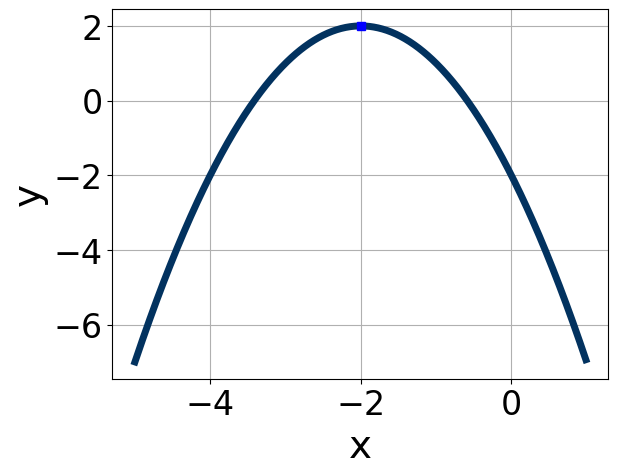
\includegraphics[width=0.5\textwidth]{../Figures/quadraticGraphToEquationC.png}
\end{center}
\begin{enumerate}[label=\Alph*.]
\item \( a \in [-1.1, -0.7], \hspace*{5mm} b \in [2, 5], \text{ and } \hspace*{5mm} c \in [-9, -3] \)
\item \( a \in [-1.1, -0.7], \hspace*{5mm} b \in [-7, -1], \text{ and } \hspace*{5mm} c \in [-4, -1] \)
\item \( a \in [-1.1, -0.7], \hspace*{5mm} b \in [2, 5], \text{ and } \hspace*{5mm} c \in [-4, -1] \)
\item \( a \in [0.2, 2.4], \hspace*{5mm} b \in [2, 5], \text{ and } \hspace*{5mm} c \in [6, 9] \)
\item \( a \in [0.2, 2.4], \hspace*{5mm} b \in [-7, -1], \text{ and } \hspace*{5mm} c \in [6, 9] \)

\end{enumerate} }
\litem{
Factor the quadratic below. Then, choose the intervals that contain the constants in the form $(ax+b)(cx+d); b \leq d.$\[ 24x^{2} +50 x + 25 \]\begin{enumerate}[label=\Alph*.]
\item \( a \in [5.98, 6.49], \hspace*{5mm} b \in [4, 10], \hspace*{5mm} c \in [3.95, 4.54], \text{ and } \hspace*{5mm} d \in [2, 9] \)
\item \( a \in [11.66, 13.4], \hspace*{5mm} b \in [4, 10], \hspace*{5mm} c \in [1.8, 2.43], \text{ and } \hspace*{5mm} d \in [2, 9] \)
\item \( a \in [-0.36, 1.49], \hspace*{5mm} b \in [13, 21], \hspace*{5mm} c \in [0.97, 1.26], \text{ and } \hspace*{5mm} d \in [23, 33] \)
\item \( a \in [1.25, 2.55], \hspace*{5mm} b \in [4, 10], \hspace*{5mm} c \in [11.85, 12.45], \text{ and } \hspace*{5mm} d \in [2, 9] \)
\item \( \text{None of the above.} \)

\end{enumerate} }
\litem{
Write the equation of the graph presented below in the form $f(x)=ax^2+bx+c$, assuming  $a=1$ or $a=-1$. Then, choose the intervals that $a, b,$ and $c$ belong to.
\begin{center}
    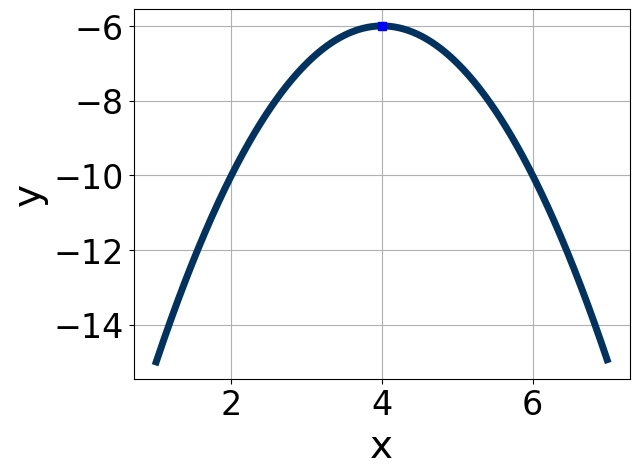
\includegraphics[width=0.5\textwidth]{../Figures/quadraticGraphToEquationCopyC.png}
\end{center}
\begin{enumerate}[label=\Alph*.]
\item \( a \in [-1.3, 0.5], \hspace*{5mm} b \in [8, 9], \text{ and } \hspace*{5mm} c \in [-23, -18] \)
\item \( a \in [0, 1.1], \hspace*{5mm} b \in [8, 9], \text{ and } \hspace*{5mm} c \in [8, 11] \)
\item \( a \in [0, 1.1], \hspace*{5mm} b \in [-8, -5], \text{ and } \hspace*{5mm} c \in [8, 11] \)
\item \( a \in [-1.3, 0.5], \hspace*{5mm} b \in [-8, -5], \text{ and } \hspace*{5mm} c \in [-23, -18] \)
\item \( a \in [-1.3, 0.5], \hspace*{5mm} b \in [-8, -5], \text{ and } \hspace*{5mm} c \in [-12, -7] \)

\end{enumerate} }
\litem{
Solve the quadratic equation below. Then, choose the intervals that the solutions belong to, with $x_1 \leq x_2$ (if they exist).\[ -12x^{2} -10 x + 4 = 0 \]\begin{enumerate}[label=\Alph*.]
\item \( x_1 \in [-1.54, -0.67] \text{ and } x_2 \in [-0.7, 1] \)
\item \( x_1 \in [-0.59, -0.03] \text{ and } x_2 \in [0.8, 1.9] \)
\item \( x_1 \in [-18.17, -17.3] \text{ and } x_2 \in [16.4, 18.4] \)
\item \( x_1 \in [-4.18, -2.99] \text{ and } x_2 \in [12.8, 13.7] \)
\item \( \text{There are no Real solutions.} \)

\end{enumerate} }
\litem{
Graph the equation below.\[ f(x) = (x-3)^2 + 18 \]\begin{enumerate}[label=\Alph*.]
\begin{multicols}{2}\item 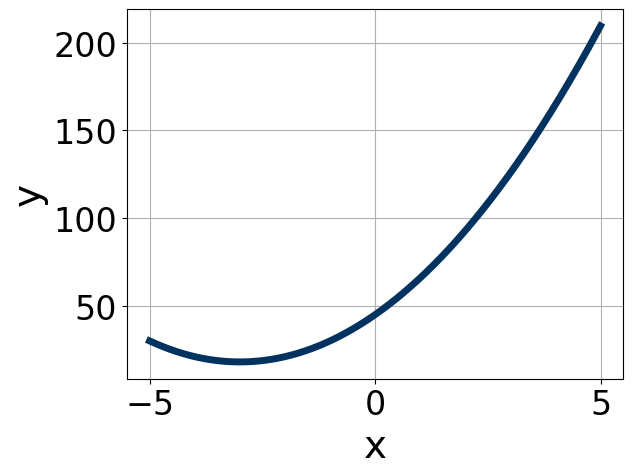
\includegraphics[width = 0.3\textwidth]{../Figures/quadraticEquationToGraphCopyAC.png}\item 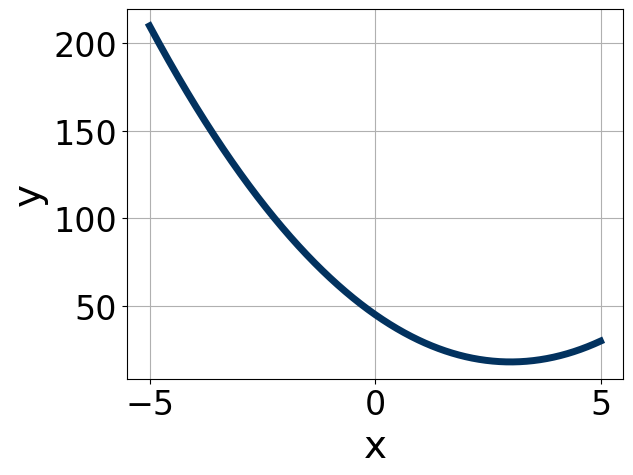
\includegraphics[width = 0.3\textwidth]{../Figures/quadraticEquationToGraphCopyBC.png}\item 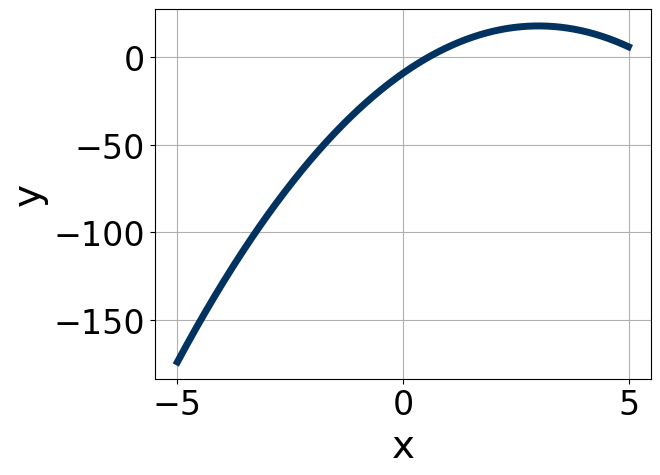
\includegraphics[width = 0.3\textwidth]{../Figures/quadraticEquationToGraphCopyCC.png}\item 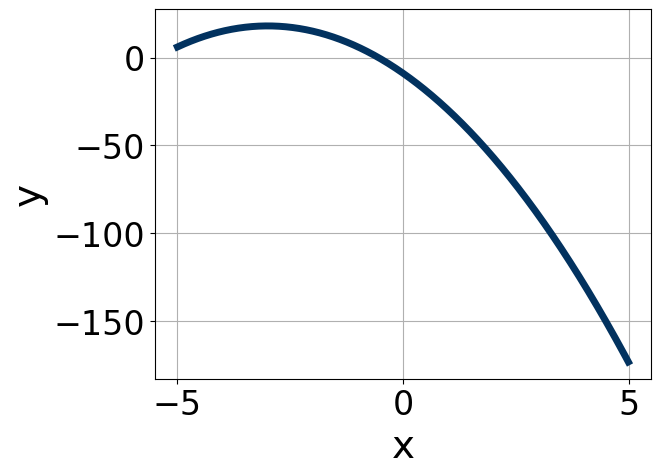
\includegraphics[width = 0.3\textwidth]{../Figures/quadraticEquationToGraphCopyDC.png}\end{multicols}\item None of the above.
\end{enumerate} }
\litem{
Solve the quadratic equation below. Then, choose the intervals that the solutions belong to, with $x_1 \leq x_2$ (if they exist).\[ -11x^{2} +7 x + 9 = 0 \]\begin{enumerate}[label=\Alph*.]
\item \( x_1 \in [-21.6, -20.4] \text{ and } x_2 \in [21.05, 22.11] \)
\item \( x_1 \in [-1.1, 1.9] \text{ and } x_2 \in [0.88, 2.39] \)
\item \( x_1 \in [-3.2, -0.8] \text{ and } x_2 \in [0.09, 0.99] \)
\item \( x_1 \in [-15.2, -12.3] \text{ and } x_2 \in [6.89, 7.07] \)
\item \( \text{There are no Real solutions.} \)

\end{enumerate} }
\litem{
Solve the quadratic equation below. Then, choose the intervals that the solutions $x_1$ and $x_2$ belong to, with $x_1 \leq x_2$.\[ 25x^{2} -75 x + 54 = 0 \]\begin{enumerate}[label=\Alph*.]
\item \( x_1 \in [0.31, 0.39] \text{ and } x_2 \in [5.96, 7.79] \)
\item \( x_1 \in [29.95, 30] \text{ and } x_2 \in [42.83, 46.12] \)
\item \( x_1 \in [0.57, 0.64] \text{ and } x_2 \in [3.3, 3.81] \)
\item \( x_1 \in [1.16, 1.25] \text{ and } x_2 \in [0.89, 2.51] \)
\item \( x_1 \in [0.4, 0.46] \text{ and } x_2 \in [4.94, 5.77] \)

\end{enumerate} }
\litem{
Solve the quadratic equation below. Then, choose the intervals that the solutions $x_1$ and $x_2$ belong to, with $x_1 \leq x_2$.\[ 25x^{2} +60 x + 36 = 0 \]\begin{enumerate}[label=\Alph*.]
\item \( x_1 \in [-3.83, -3.59] \text{ and } x_2 \in [-0.46, -0.32] \)
\item \( x_1 \in [-6.78, -5.74] \text{ and } x_2 \in [-0.37, -0.09] \)
\item \( x_1 \in [-30.58, -29.25] \text{ and } x_2 \in [-30.05, -29.91] \)
\item \( x_1 \in [-1.75, -0.99] \text{ and } x_2 \in [-1.23, -1.11] \)
\item \( x_1 \in [-2.56, -2.16] \text{ and } x_2 \in [-0.79, -0.53] \)

\end{enumerate} }
\litem{
Graph the equation below.\[ f(x) = -(x-3)^2 + 17 \]\begin{enumerate}[label=\Alph*.]
\begin{multicols}{2}\item 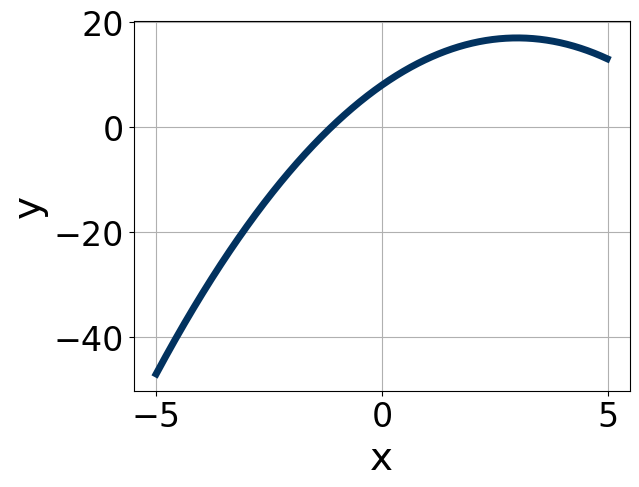
\includegraphics[width = 0.3\textwidth]{../Figures/quadraticEquationToGraphAC.png}\item 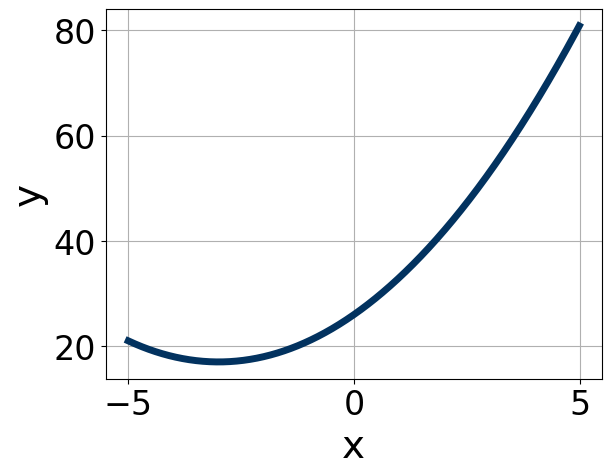
\includegraphics[width = 0.3\textwidth]{../Figures/quadraticEquationToGraphBC.png}\item 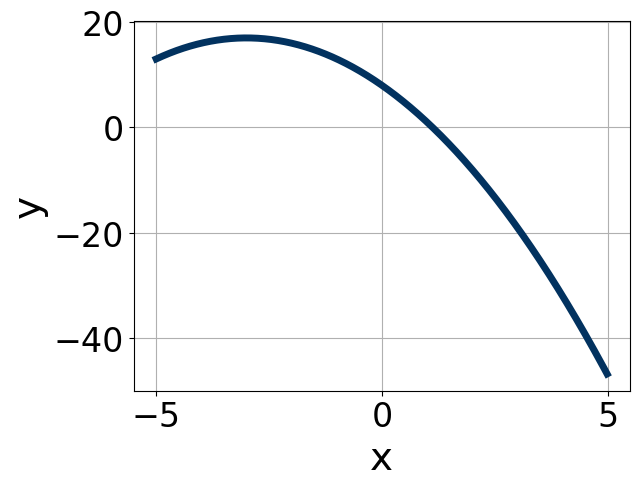
\includegraphics[width = 0.3\textwidth]{../Figures/quadraticEquationToGraphCC.png}\item 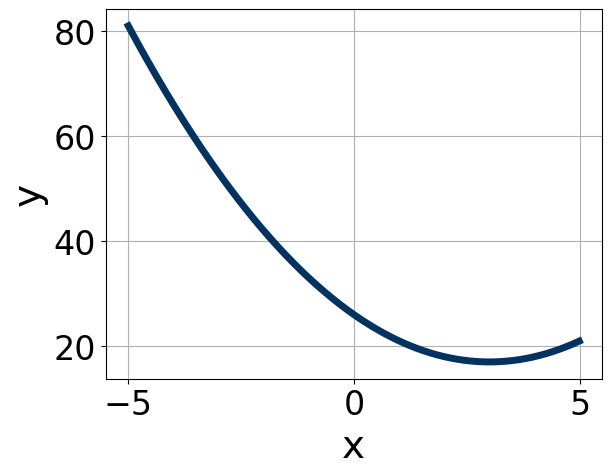
\includegraphics[width = 0.3\textwidth]{../Figures/quadraticEquationToGraphDC.png}\end{multicols}\item None of the above.
\end{enumerate} }
\end{enumerate}

\end{document}